\documentclass[a4paper,12pt]{article} % Document class

% Packages
\usepackage[utf8]{inputenc} % Encoding
\usepackage{amsmath} % For mathematical formulas
\usepackage{amsfonts} % For math fonts
\usepackage{graphicx} % For including images
\usepackage{hyperref} % For hyperlinks
\usepackage{geometry} % For page dimensions
\usepackage{natbib} % For bibliography management
\usepackage{graphicx} % For including images
\usepackage{rotating} % For sideways tables and figures
\usepackage[table,xcdraw]{xcolor} % For colored tables
\usepackage{colortbl} % For colored tables
\usepackage{array} % For advanced table formatting
\usepackage{float} % For [H] positioning

% Colors for tables
\definecolor{maternal_dem}{HTML}{FFDDDD} % light red
\definecolor{father_char}{HTML}{D5E8D4} % light green
\definecolor{health_risk}{HTML}{DDDDFF} % light blue
\definecolor{prenatal_care}{HTML}{FFFFCC} % light yellow
\definecolor{smoking_use}{HTML}{FFCCFF} % light magenta
\definecolor{anthropometrics}{HTML}{CCFFFF} % light cyan
\definecolor{pregnancy_hist}{HTML}{FFE5CC} % peach
\definecolor{Infections}{HTML}{E0CCFF} % light purple
\definecolor{labor}{HTML}{CCE5FF} % soft blue
\definecolor{infant}{HTML}{D5FFCC} % mint green
\definecolor{cog_anomal}{HTML}{FFFFFF} % pink
\definecolor{maternal_mortality}{HTML}{BBBBBB} % lavender


% Page dimensions
\geometry{margin=1in} % Set margins

\title{Causal Inference - project proposal \\ Breastfeeding and Infant Mortality} % Title of the document
\author{Noam Sasson - 214439929 \& Alon Eitan - 214304693} % Author's name
\date{\today} % Date

\begin{document} % Start of the document

\maketitle % Create the title
\section{Causal Question} % Section
The causal question is: \textit{Does breastfeeding during early stages of life affect infant mortality during the first year of life?}
\section{Previous Knowledge On the Topic}
\begin{enumerate}
    \item Time to initiation of breastfeeding and neonatal mortality and morbidity: a systematic review (\cite{AmandaK2013}) -  reporting a direct association between early breastfeeding initiation and neonatal mortality and morbidity outcomes.
    \item Delayed breastfeeding initiation and infant survival: A systematic review and meta-analysis (\cite{EmilyR2015}) - Compared to infants who initiated breastfeeding $\leq$ 1 hour after birth, infants who initiated breastfeeding 2-23 hours after birth had a 33\% greater risk of neonatal mortality.
    \item Infant and young child feeding, a WHO fact sheet (\cite{who2021}) - Highly recommends early initiation of breastfeeding within the first hour of life.
\end{enumerate}
\section{Data We Intend To Use}
We chose the 2015 Cohort Linked Birth/Infant Death Data Set from the site of the \textbf{National Center for Health Statistics}.
The data contains records of all babies with birth certificates born in the United States In the year 2015, and their survival status for their first year (whether they died within 2015 or 2016).
All the enteries of each record are the birth certificates that were filled on the birth of the baby, linked with the infant death certificates that were filled on the death of the baby (only if baby died), with additional questions that the patients were asked. \newline
\begin{center}
\textit{"The National Center for Health Statistics is the nation's source for official health statistics. We collect, analyze, and share data and statistics to guide programs and policies that improve the health of people across the United States."}
\end{center}
% Previous research has established strong associations between breastfeeding practices and infant health outcomes. \citet{ehp2004} provides evidence on the relationship between breastfeeding and babies' health and survival. Furthermore, \citet{tamiru2015} conducted a longitudinal study in Northwest Ethiopia, demonstrating that exclusive breastfeeding is the strongest predictor of infant survival in their study population. Additionally, \citet{sankar2015} performed a comprehensive systematic review and meta-analysis examining optimal breastfeeding practices and their impact on infant and child mortality, providing robust evidence for the protective effects of breastfeeding.
\section{Causal Assumptions} % Section
The infant mortality dataset contains a lot of information about the mother's and father's background and status, and the infant's health. \newline
From the vast amount of features to select from, we collected $\sim$ 100 features spanning over 12 categories, which we believe are relevant to the causal question. \newline
\textbf{1.} Maternal Demographics, \textbf{2.} Father Paternal Characteristics, \textbf{3.} Maternal Health \& Risk Factors, \textbf{4.} Prenatal Care, \textbf{5.} Smoking / Tobacco Use, \textbf{6.} Anthropometrics / Weight, \textbf{7.} Pregnancy History, \textbf{8.} Infections, \textbf{9.} Labor \& Delivery, \textbf{10.} Infant \& Birth Outcomes, \textbf{11.} Congenital Anomalies of the Newborn, \textbf{12.} Maternal Mortality Features
% \begin{enumerate}
%     \item Maternal Demographics
%     \item Father Paternal Characteristics
%     \item Maternal Health \& Risk Factors
%     \item Prenatal Care
%     \item Smoking / Tobacco Use
%     \item Anthropometrics / Weight
%     \item Pregnancy History
%     \item Infections
%     \item Labor \& Delivery
%     \item Infant \& Birth Outcomes
%     \item Congenital Anomalies of the Newborn
%     \item Maternal Mortality Features
% \end{enumerate}

% \begin{table}[h!]
% \centering
% \caption{Selected Features by Category}
% \label{tab:features}
% \tiny
% \begin{tabular}{|p{1.5cm}|p{1.5cm}|p{1.8cm}|p{1.2cm}|p{1.5cm}|p{1.5cm}|p{1.4cm}|p{1cm}|p{1.3cm}|p{1.5cm}|p{1.4cm}|p{1.3cm}|}
% \hline
% \textbf{Maternal Demographics} & \textbf{Paternal Characteristics} & \textbf{Maternal Health \& Risk Factors} & \textbf{Prenatal Care} & \textbf{Smoking / Tobacco Use} & \textbf{Anthropometrics / Weight} & \textbf{Pregnancy History} & \textbf{Infections} & \textbf{Labor \& Delivery} & \textbf{Infant \& Birth Outcomes} & \textbf{Congenital Anomalies} & \textbf{Maternal Morbidity} \\
% \hline
% MAGER & FAGECOMB & RF\_PDIAB & PRECARE & CIG\_0 & MHTR & LBO\_REC & IP\_GON & LD\_INDL & SEX & CA\_ANEN & MM\_MTR \\
% MRACE31 & FRACE31 & RF\_GDIAB & PREVIS & CIG\_1 & BMI & TBO\_REC & IP\_SYPH & LD\_AUGM & COMBGEST & CA\_MNSB & MM\_PLAC \\
% MEDUC & FEDUC & RF\_PHYPE & & CIG\_2 & BMI\_R & PRIORLIVE & IP\_CHLAM & LD\_CHOR & GESTREC10 & CA\_CCHD & MM\_RUPT \\
% DMAR & & RF\_GHYPE & & CIG\_3 & PWgt\_R & PRIORDEAD & IP\_HEPB & LD\_STER & GESTREC3 & CA\_CDH & MM\_UHYST \\
% MBSTATE\_REC & & RF\_EHYPE & & CIG\_REC & DWgt\_R & PRIORTERM & IP\_HEPC & LD\_ANTB & BWTR14 & CA\_OMPH & MM\_AICU \\
% RESTATUS & & RF\_PPB & & & WTGAIN & ILLB\_R & NO\_INFEC & LD\_ANES & APGAR5 & CA\_GAST & NO\_MMORB \\
% WIC & & RF\_INFT & & & WTGAIN\_REC & ILLB\_R11 & & ME\_PRES & APGAR10 & CA\_LIMB & \\
% PAY & & RF\_DRG & & & & ILOP\_R & & ME\_ROUT & DPLURAL & CA\_CLEFT & \\
% & & RF\_ART & & & & ILOP\_R11 & & ME\_TRIAL & SETORDER\_R & CA\_CLPAL & \\
% & & RF\_CESAR & & & & ILP\_R & & DMETH\_REC & AB\_AVEN1 & CA\_DOWN & \\
% & & RF\_CESARN & & & & ILP\_R11 & & RDMETH\_REC & AB\_AVEN6 & CA\_DISOR & \\
% & & NO\_RISKS & & & & & & & AB\_NICU & CA\_HYPO & \\
% & & & & & & & & & AB\_SURF & NO\_CONGEN & \\
% & & & & & & & & & AB\_ANTI & & \\
% & & & & & & & & & AB\_SEIZ & & \\
% & & & & & & & & & NO\_ABNORM & & \\
% \hline
% \end{tabular}
% \end{table}

\begin{table}[H]
\centering
\caption{Features Dictionary for Infant Mortality Analysis}
\label{tab:features_dictionary}
\small
\begin{tabular}{|>{\columncolor{maternal_dem}}l|>{\columncolor{father_char}}l|}
\hline
\textbf{Maternal Demographics (mother)} & \textbf{Paternal Characteristics (father)} \\
\hline
MAGER -  Mother’s Age Recode 41& FAGECOMB -  Father’s Combined Age (Revised)\\
MRACE31 -  Mother’s Race Recode 31& FRACE31 -  Father’s Race Recode 31\\
MEDUC -  Mother’s Education& FEDUC -  Father’s Education\\
DMAR -  Marital Status&  \\
MBSTATE\_REC -  Mother’s Nativity&  \\
RESTATUS -  Residence Status&  \\
WIC -  participation in WIC program&  \\
PAY -  Payment Source&  \\
\hline
\end{tabular}
\end{table}

\begin{table}[H]
\centering
% \caption{Features Dictionary for Infant Mortality Analysis}
% \label{tab:features_dictionary}
\small
\begin{tabular}{|>{\columncolor{health_risk}}l|>{\columncolor{prenatal_care}}l|}
\hline
\textbf{Maternal Health \& Risk Factors} & \textbf{Prenatal Care} \\
\hline
RF\_PDIAB -  Pre-pregnancy Diabetes& PRECARE -  Month Prenatal Care\\
RF\_GDIAB -  Gestational Diabetes& PREVIS -  Number of Prenatal Visits (Revised)\\
RF\_PHYPE -  Pre-pregnancy Hypertension&  \\
RF\_GHYPE -  Gestational Hypertension&  \\
RF\_EHYPE -  Hypertension Eclampsia&  \\
RF\_PPB -  Previous Preterm Birth&  \\
RF\_INFT -  Infertility Treatment&  \\
RF\_DRG -  Fertility Enhancing Drugs&  \\
RF\_ART -  Assisted Reproductive Technology&  \\
RF\_CESAR -  Previous Cesareans&  \\
RF\_CESARN -  Number of Previous Cesareans&  \\
NO\_RISKS -  No Risk Factors Checked&  \\
\hline
\end{tabular}
\end{table}

\begin{table}[H]
\centering
% \caption{Features Dictionary for Infant Mortality Analysis}
% \label{tab:features_dictionary}
\small
\begin{tabular}{|>{\columncolor{smoking_use}}l|>{\columncolor{anthropometrics}}l|}
\hline
\textbf{Smoking / Tobacco Use} & \textbf{Anthropometrics / Weight} \\
\hline
CIG\_0 -  Cigarettes Before Pregnancy Recode& MHTR -  Mother’s Height in Inches (Recode)\\
CIG\_1 -  Cigarettes 1st Trimester Recode& BMI -  BMI\\
CIG\_2 -  Cigarettes 2nd Trimester Recode& BMI\_R -  Body Mass Index Recode\\
CIG\_3 -  Cigarettes 3rd Trimester Recode& PWgt\_R -  Pre-pregnancy Weight Recode\\
CIG\_REC -  Cigarette Recode (Revised)& DWgt\_R -  Delivery Weight Recode\\
 & WTGAIN -  Weight Gain\\
 & WTGAIN\_REC -  Weight Gain Recode\\
\hline
\end{tabular}
\end{table}

\begin{table}[H]
\centering
% \caption{Features Dictionary for Infant Mortality Analysis}
% \label{tab:features_dictionary}
\small
\begin{tabular}{|>{\columncolor{pregnancy_hist}}l|>{\columncolor{Infections}}l|}
\hline
\textbf{Pregnancy History} & \textbf{Infections} \\
\hline
LBO\_REC -  Live Birth Order Recode& IP\_GON -  Gonorrhea\\
TBO\_REC -  Total Birth Order Recode& IP\_SYPH -  Syphilis\\
PRIORLIVE -  Prior Births Now Living& IP\_CHLAM -  Chlamydia\\
PRIORDEAD -  Prior Births Now Dead& IP\_HEPB -  Hepatitis B\\
PRIORTERM -  Prior Other Terminations& IP\_HEPC -  Hepatitis C\\
ILLB\_R -  Interval of Last Live Birth Recode& NO\_INFEC -  No Infections Checked\\
ILLB\_R11 -  Interval of Last Live Birth Recode 11&  \\
ILOP\_R -  Interval of Last Other Pregnancy Recode&  \\
ILOP\_R11 -  Interval of Last Other Pregnancy Recode 11&  \\
ILP\_R -  Interval of Last Pregnancy Recode&  \\
ILP\_R11 -   Interval of Last Pregnancy Recode 11&  \\
\hline
\end{tabular}
\end{table}

\begin{table}[H]
\centering
% \caption{Features Dictionary for Infant Mortality Analysis}
% \label{tab:features_dictionary}
\small
\begin{tabular}{|>{\columncolor{labor}}l|>{\columncolor{infant}}l|}
\hline
\textbf{Labor \& Delivery} & \textbf{Infant \& Birth Outcomes} \\
\hline
LD\_INDL -  Induction of Labor& SEX -  sex of infant\\
LD\_AUGM -  Augmentation of Labor& COMBGEST -  Combined Gestation Imputed\\
LD\_CHOR -  Chorioamnionitis& GESTREC10 -  Combined Gestation Recode 10\\
LD\_STER -  Steroids& GESTREC3 -  Combined Gestation Recode 3\\
LD\_ANTB -  Antibiotics& BWTR14 -  Birth Weight Recode 14\\
LD\_ANES -  Anesthesia& APGAR5 -  Five Minute APGAR Score\\
ME\_PRES -  Fetal Presentation& APGAR10 -  Ten Minute APGAR Score\\
ME\_ROUT -  Final Route \& Method of Delivery& DPLURAL -  Plurality Recode\\
ME\_TRIAL -  Trial of Labor Attempted& SETORDER\_R -  Set Order Recode\\
DMETH\_REC -  Delivery Method Recode& AB\_AVEN1 -  Assisted Ventilation\\
RDMETH\_REC -  Delivery Method Recode Combined& AB\_AVEN6 -  Assisted Ventilation \textgreater  6 hrs\\
 & AB\_NICU -  Newborn Admitted to NICU\\
 & AB\_SURF -  Newborn Received Surfactant Therapy\\
 & AB\_ANTI -  Newborn Received Antibiotics\\
 & AB\_SEIZ -  Newborn Experienced Seizures\\
 & NO\_ABNORM -  No Abnormal Conditions Checked\\
\hline
\end{tabular}
\end{table}

\begin{table}[H]
\centering
% \caption{Features Dictionary for Infant Mortality Analysis}
% \label{tab:features_dictionary}
\small
\begin{tabular}{|>{\columncolor{cog_anomal}}l|>{\columncolor{maternal_mortality}}l|}
\hline
\textbf{Congenital Anomalies of the Newborn} & \textbf{Maternal Mortality Features} \\
\hline
CA\_ANEN -  Anencephaly& MM\_MTR -  Maternal Transfusion\\
CA\_MNSB -  Meningomyelocele / Spina Bifida& MM\_PLAC -  Perineal Laceration\\
CA\_CCHD -  Cyanotic Congenital Heart Disease& MM\_RUPT -  Ruptured Uterus\\
CA\_CDH -  Congenital Diaphragmatic Hernia& MM\_UHYST -  Unplanned Hysterectomy\\
CA\_OMPH -  Omphalocele& MM\_AICU -  Admission to Intensive Care\\
CA\_GAST -  Gastroschisis& NO\_MMORB -  No Maternal Morbidity Checked\\
CA\_LIMB -  Limb Reduction Defect&  \\
CA\_CLEFT -  Cleft Lip with or without Cleft Palate&  \\
CA\_CLPAL -  Cleft Palate Alone&  \\
CA\_DOWN -  Down Syndrome&  \\
CA\_DISOR -  Suspected Chromosomal Disorder&  \\
CA\_HYPO -  Hypospadias&  \\
NO\_CONGEN -  No Congenital Anomalies Checked&  \\
\hline
\end{tabular}
\end{table}


The causal assumptions we intend to use are mapped in the following causal DAG:

\begin{center}
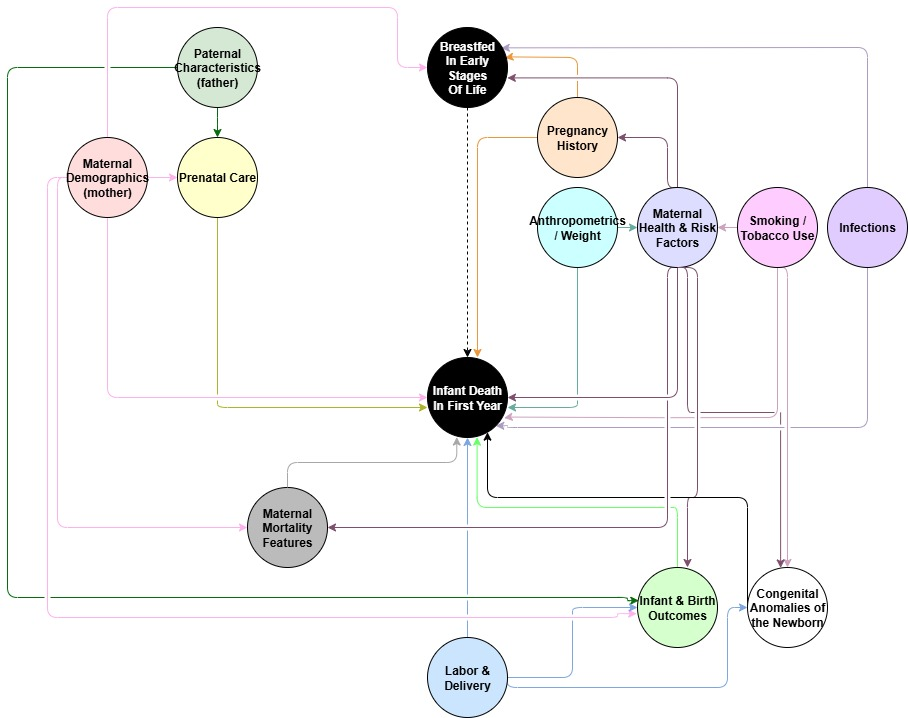
\includegraphics[width=0.8\textwidth]{causal_graph.jpg}
\end{center}

\section{Challenges}

\begin{enumerate}
    \item Confounding Variables \\\\
    The primary challenge is to isolate the effect of early breastfeeding from numerous confounding variables that influence both the mother's decision to breastfeed and the infant's health outcomes. The project's extensive feature list and causal DAG highlight many of these factors, including:
        \begin{itemize}
            \item Socioeconomic and Demographic Factors: Maternal demographics like age (MAGER), race (MRACE), and education (MEDUC) are likely correlated with both breastfeeding and infant mortality. Paternal characteristics, such as age (FAGECOMB) and education (FEDUC), are also included as potential confounders.
            \item Maternal Health and History: The mother's pre-existing health conditions, such as diabetes (RF\_PDIAB) or hypertension (RF\_PHYPE), her pregnancy history (e.g., previous preterm births), and health during pregnancy (e.g., gestational diabetes) are significant confounders. These factors can affect a mother's ability to breastfeed and are also directly related to infant health.
            \item Prenatal Care: The number of prenatal visits (PREVIS) and the month prenatal care began (PRECARE) are key confounders as they reflect a mother's access to and engagement with healthcare, which can influence both early breastfeeding support and infant outcomes.
            \item Smoking/Tobacco Use: The amount of cigarettes smoked before and during pregnancy (CIG\_0, CIG\_1, CIG\_2, CIG\_3) is a known risk factor for poor infant health and may be associated with breastfeeding decisions, making it a critical confounder to control for.
        \end{itemize}
    \item Reverse Causality and Endogeneity\\\\
        The analysis may be affected by reverse causality, where the infant's health status influences the mother's ability or decision to breastfeed, rather than the other way around. For example, a newborn with a congenital anomaly (e.g., Down Syndrome or Cleft Palate) may have difficulty breastfeeding, and this condition also increases the risk of mortality. This relationship is depicted in the causal DAG, with an arrow from :Congenital Anomalies of the Newborn: to :Infant Death in first year:. Similarly, :Infant \& Birth Outcomes: like low birth weight (BWTR14) and low Apgar scores (APGAR5) could affect breastfeeding. This endogeneity makes it challenging to disentangle the true causal effect of breastfeeding.  
    \item Causal Inference from Observational Data\\\\
    The project relies on an infant mortality dataset, which is a form of observational data. Because a randomized controlled trial is not possible for ethical reasons, establishing a causal link requires careful statistical methods to control for observed and unobserved confounding. While the provided project outlines a detailed plan to use a large number of features and a causal DAG to map relationships, there remains the risk of unobserved confounding variables that are not captured in the dataset. This could lead to biased estimates of the effect of breastfeeding.

\end{enumerate}

\section{Estimation Methods}
Our goal is to estimate the ATE of breastfeeding on infant mortality during the first year of life (target variable is probability of death in the first year).
We are going to use the following estimation methods shown in the course:
\begin{enumerate}
    \item Matching: We will use matching techniques seen in the course (k-nearest neighbor matching and propensity score matching).
    \item T-learner \& S-Learner: specificaly using 
    \begin{itemize}
        \item  Logistic Regression both trained with IPW to handle treatment label imbalance (IPW Derived from a learned propensity model).
        \item  Neural Networks (NN) with similar IPW training, or smart balanced sampling from both treatment and control groups during training.
    \end{itemize}
   
\end{enumerate}

\section{Robustness Checks}
To evaluate the reliability of our causal estimates, we will conduct a series of robustness checks, testing our matching, T-learner, and S-learner models.\\\\
For the matching approach, we will examine the stability of our findings by varying key parameters. This includes exploring different caliper widths, adjusting the number of matches used for each treated unit, and employing alternative distance metrics, such as the Mahalanobis distance. Consistency in the estimated treatment effect across these variations will serve as a strong indicator of the model's stability.\\\\
For the meta-learners, including the T-learner and S-learner, a crucial robustness check will involve assessing the dependence of our results on the choice of the underlying base learners. We will compare the causal estimates obtained from different regularization functions for the Logistic Regression, and same for another learner such as Random Forest - consistent Results on the 3 models (Logistic Regression, Random Forest and NN) will indicate a significant ATE.\\\\
% We will also perform a thorough analysis of covariate balance both before and after matching, as well as within the meta-learner frameworks, to confirm that the assumptions of each method are met. 
Together, these multifaceted checks will provide confidence that our causal estimates are robust to different modeling choices and potential sources of uncertainty.

% do 3,7
\bibliographystyle{plainnat}
\bibliography{references} % Bibliography
\end{document} % End of the document